\subsection{Métodología de experimentación}
En esta sección desarrollaremos los experimentos planteados, desde la generación de instancias de prueba hasta los criterios de medición utilizados y los detalles de los experimentos.
%\subsubsection{Consideraciones iniciales}
%\begin{itemize}
%    \item La pared interna del horno en teoría debería ser de 1500 grados constantes, nosotros consideramos más realista que al variar los ángulos de la pared interna, la temperatura varíe uniformemente entre $1500 \pm \epsilon$, con $\epsilon = 50$ .
%
%    \item Respecto a las temperaturas externas, varian entre 50 y 200 de manera aleatoria uniforme en los experimentos presentados a continuacion.
%\end{itemize}
%
%\subsubsection{Generación de casos de prueba}
%Los casos de prueba son generados mediante un script de python llamado testgen.py, dentro de la carpeta tools. El mismo posee 3 modos de ejecuci\'on: 
%\begin{enumerate}
%    %\item \textbf{Modo 1:} Dados por par\'ametro un radio interno, externo e isoterma fijas, toma adem\'as  una cantidad de radios inicial, una final, una cantidad de \'angulos inicial, una final, y para cada combinaci\'on de cantidades de ellos genera un n\'umero de instancias tambi\'en provisto por par\'ametro. En cada instancia, las temperaturas internas y externas son generadas pseudoaleatoriamente, ejecutando el comando \textbf{random.uniform(1450, 1550)} para las temperaturas internas y \textbf{random.uniform(50, 200)}.
%    %\item \textbf{Modo 2:} Dados un radio interno, externo, isoterma, n\'umero de \'angulos y radios fijos por par\'ametro, genera un \'unico archivo en el que var\'ia las temperatura de esa discretizaci\'on particular (usando los comandos descriptos anteriormente), generando un n\'umero de instancias provisto por par\'ametro.
%    \item \textbf{Modo 3:} Dados un radio interno, externo, isoterma, y n\'umero de ángulos fijos por par\'ametro, se le especifica una cantidad de radios inicial y una final.  Para cada cantidad de radios genera un \'unico vector de temperaturas internas y externas, y genera tantas instancias como se le especifique.
%
%\end{enumerate}
%\textbf{Nota: } Para algunos experimentos consideramos apropiado fijar las temperaturas externas en 1500 y las internas en 100.

\subsubsection{Métricas de performance}

Se medir\'a y comparar\'a la performance de ambos m\'etodos en la resoluci\'on de diversas instancias del problema. El tiempo se mide en microsegundos, y corresponde al tiempo de procesamiento de CPU, dejando fuera de consideraci\'on el tiempo de entrada/salida. El objetivo \'ultimo es encontrar una relaci\'on entre la complejidad te\'orica de ambos algoritmos y su tiempo de c\'omputo, y realizar la comparaci\'on de ambos m\'etodos en distintos escenarios. Todos los casos considerados est\'an especificados en la secci\'on \textbf{Esquema de experimentaci\'on}. En todos los casos se mide el tiempo total de resolucion en CPU de \textbf{todas} las instancias del archivo de entrada.

\subsubsection{Método de posiciónamiento estimado de la isoterma}
El problema consiste en estimar, para cada ángulo, la posición radial de la isoterma \texttt{$\alpha$}.\\
Consideremos la función \textbf{contínua} de temperatura $T(r,\theta)$ definida sobre las coordenadas polares $r,\theta$. Si fijamos $\theta = \theta_i$ podemos definir la función $g_{\theta_i}(r) = T(r,\theta_i)$ como la función de temperatura sobre todos los radios \textbf{contínuos} del ángulo $\theta_i$ fijado. Dado que nosotros conocemos $m+1$ puntos aproximados de dicha función, esto reduce el problema a aproximar el elemento $ z_\alpha \in Dom(g_{\theta_i}) = { [R_i \dots R_e] }$ tal que $g_{\theta_i}(z_\alpha) = \alpha$. \\
El método propuesto consiste en aplicar el siguiente algoritmo a las aproximaciones discretas conocidas de las funciones $g_{\theta_i}$, para todos los ángulos.

\begin{proposition}[Algoritmo de estimación de la isoterma k por ajuste lineal]
    Sea $\hat{g_{\theta_i}}$ la función \textbf{discreta de aproximaciones} de temperatura de un ángulo i.
    \begin{enumerate}
        \item Buscar $ x_1, x_2 \in Dom(\hat{g_{\theta_i}}) $ tales que $ \hat{g_{\theta_i}}(x_1) \leq \alpha \leq \hat{g_{\theta_i}}(x_2)$ y esta cota sea ajustada.
        
        \item $z_\alpha = x_1 + \left(\frac{x_2 - x_1}{\hat{g_{\theta_i}}(x_2) - \hat{g_{\theta_i}}(x_1)}\right) * (\alpha - \hat{g_{\theta_i}}(x_1))$

        \item Devolver $z_\alpha$.
    \end{enumerate}
    $z_\alpha$ es la posición estimada linealmente de la isoterma tal que $g_{\theta_i}(z_\alpha) = \alpha$.
\end{proposition}

\begin{proposition}[Dominio de correctitud de la estimación]
    El algoritmo anterior estima linealmente la isoterma $\alpha$ entre $x_1$ y $x_2$ si:
    \begin{itemize}
        \item $\displaystyle\min_{x \in Dom(\hat{g_{\theta_i}})}{\hat{g_{\theta_i}}(x)} \leq \alpha \leq \displaystyle\max_{x \in Dom(\hat{g_{\theta_i}})}{\hat{g_{\theta_i}}(x)}$.
        \item $\alpha \notin Im(\hat{g_{\theta_i}})$.
    \end{itemize}
    \begin{itemize}
        \item En caso de que $\alpha$ esté fuera del rango $[min..max]$ por convención se establece que la isoterma se encuentra en una posición radial $R_i - \epsilon$ o $R_e + \epsilon$ según corresponda.
        \item En caso de que $\alpha \in Im(\hat{g_{\theta_i}})$ entonces $z = x_1 = x_2$ y no es necesario ajuste lineal.
    \end{itemize}
\end{proposition}
\begin{proposition}[Idea intuitiva de la correctitud del algoritmo de estimacion lineal]
    Si se cumplen las hipótesis de la proposición anterior entonces la cota existe y el algoritmo procederá a hacer el cálculo aproximado del paso siguiente, que no es más que un ajuste lineal entre los dos puntos de las cotas. Es decir, estamos asumiendo que el calor se disipa linealmente entre 2 puntos cualesquiera de la función.\\
    \vspace{0.3cm}
    \textbf{Nota:} Asumir esto no es necesariamente correcto, se podría hacer un analisis más fino graficando las funciones $g_{\theta_i}$ y aplicando métodos más avanzados de estimación para que la curva quede más suave. Por simplicidad solo consideramos el ajuste lineal en este trabajo.
\end{proposition}

\subsubsection{Métricas de seguridad de la isoterma}
Plantemos una métrica que estima la \texttt{estabilidad} o \texttt{seguridad} de la pared del horno estableciendo una relacion relativa entre la posición de la isoterma y el radio externo. 
\begin{proposition}[Métrica de seguridad del horno basada en la posición relativa de la isoterma] Sea $iso_\alpha$ la solucion del sistema, es decir, el conjunto de radios para cada angulo que indica la posicion radial de la isoterma.\\
    Consideremos $\Delta_{iso_\alpha} = \left( \frac{f(iso_\alpha) - R_i}{R_e - R_i} \right)$, donde $f(iso_\alpha)$ es una función de la isoterma, en nuestro caso, consideramos que el máximo o el promedio son buenas métricas.\\
    Salvo casos patológicos, vale que $0 \leq \Delta_{iso_\alpha}\leq 1$. Luego basta establecer un \textbf{límite de seguridad} $0 \leq \gamma_0 \leq 1$ tal que si vale $\Delta_{iso_\alpha} > \gamma_0$ se considera \texttt{inestable} o \texttt{insegura} la pared del horno.
\end{proposition}

\subsection{Esquema de experimentación}
\subsubsection{Experimentos focalizados en la performance}

\begin{proposition}[La performance es invariante bajo cambios de datos iniciales cualitativos del problema] La variacion de las condiciones iniciales del problema, es decir, temperaturas internas y externas no cambian el tiempo de resolucion del sistema de ecuaciones.(Utilizando los algoritmos estandares sin optimizaciones). Esto se debe a que la matriz resultante no cambia su dimension al cambiar estos parametros y la complejidad de los algoritmos reside en el tamaño de la matriz y no sus elementos.
\end{proposition}

\begin{proposition}[Relacion entre variables de la discretizacion y tamaño de la matriz del sistema] La performance de los algoritmos se puede medir incrementando las variables (n, m+1) del problema conjuntamente.
\end{proposition}

 Dado que en la seccion de desarrollo especificamos que $A \in \mathbb{R}^{n(m+1)\times n(m+1)}$ donde n y $m+1$ representan los parametros de la discretizacion. Tenemos que la dimension de la matriz es $n(m+1)\times n(m+1)$. Ademas, sabemos que los algoritmos tienen una complejidad teorica definida sobre una variable $k = n(m+1)$, que expresa el tamaño de una matriz cuadrada $A \in \mathbb{R}^{k\times k}$ (ie. LU y Gauss son $\mathcal{O}(k^3)$), luego podemos afirmar que la complejidad teorica de gauss y lu se puede escribir como $\mathcal{O}((n*(m+1))^3) = \mathcal{O}((n*m + n))^3) = \mathcal{O}((n*m)^3) $ pues ($m\geq1$). \\
 Veamos como se comporta la funcion $z = n*m$ con valores de $n, m$ en el rango $[10..80]$.\\

\begin{center}
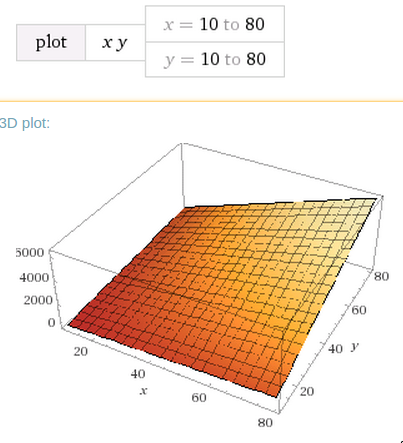
\includegraphics[scale=0.65]{img/nTimesM-3dPlot.png}
\end{center}

En el grafico puede verse, que fijando n y variando m, o al reves, se obtiene un crecimiento lineal en esa direccion. Asimismo, variando n y m al mismo tiempo, se obtiene un crecimiento lineal por la diagonal entre $(0,0)$ y $(80,80)$

Dado que nosotros queremos ver como se comportan los algoritmos cuando $k = m*n$ aumenta, nos parece representativo solo tomar combinaciones de $n, m$ que varien conjuntamente, es decir, movernos por la diagonal del plano entre $(0, 0)$ y $(n_{max}, m_{max})$.
\vspace{0.3cm}

Los experimentos de performance se dividen en dos secciones:

\begin{enumerate}

\item \textbf {Performance de los m\'etodos en funci\'on de la discretizaci\'on para una instancia:}  Se generaron diversas discretizaciones del problema, variando la cantidad de radios y angulos, conjuntamente, de 5 a 60, con una instancia para cada discretizaci\'on. El objetivo es analizar la evoluci\'on del tiempo de c\'omputo a mayor granularidad de la discretizaci\'on, y comprobar emp\'iricamente que la complejidad de ambos algoritmos es del orden c\'ubico. Asimismo, factorizacion LU deberia tomar mas tiempo pues su constante es mas grande al realizar mas operaciones que simple triangulación.

\item \textbf{Performance de EG vs LU variando la cantidad de instancias y la granularidad de la discretizacion: } Para varias cantidades de instancias por archivo de test, se generan muchas discretizaciones diferentes. El objetivo de este test es analizar que ocurre con el tiempo de ejecución cuando se resuelven muchas instancias utilizando EG o LU. Tambien se evalua la influencia de las diferentes discretizaciones para cada cantidad de instancias.

\end{enumerate}

\subsubsection{Diferencia numérica de soluciones entre EG y LU}
El objetivo de estos experimentos es analizar la diferencia numérica de la solución de un determinado sistema con EG y LU. Lo que nos va a interesar ver es distintas métricas de \texttt{distancia} entre dos soluciones $\hat{x} , x$ para el mismo sistema $Ax=b$, resueltas con EG y LU. Consideramos para estos experimentos, variar el tamaño de la matriz A, usando el mismo criterio que en la sección de performance, variando n y m al mismo tiempo.

\vspace{0.3cm}

Métricas de distancia utilizadas:
\begin{itemize}
    \item $\norm{ x - \hat{x} }_\infty$: distancia maxima entre $x$ y $\hat{x}$
    \item $\norm{ x - \hat{x} }_2$ : distancia euclídea entre $x$ y $\hat{x}$
\end{itemize}

\textbf{Nota: } Las temperaturas externas(1500) e internas(100) son \textbf{constantes} en todos los tests. 

\subsubsection{Evolución de la temperatura y posición de la isoterma con distintas discretizaciones}

El objetivo de los experimentos planteados en esta sección es analizar la posicion de la isoterma a medida que se varían las discretizaciones en diferentes direcciones(radios, angulos y ambas al mismo tiempo.). Para realizar esto, necesitamos que cada test de un experimento \textbf{tenga la misma solución}. Todos los experimentos mencionados debajo comienzan con una discretización gruesa y se van afinando a medida que crece la componente correspondiente(según el experimento). Se espera que la posicion de la isoterma \texttt{converja} a la posicion \texttt{real}.

\begin{proposition}[Convergencia de la solucion] Dado que estamos aproximando una función contínua con discretizaciones, asumimos que si hacemos $n \to\infty \land m\to\infty$, la solucion obtenida se parece cada vez a la solucion \texttt{real}. En otras palabras, la posición de la isoterma converge.
\end{proposition}

Para corroborar esta proposición tomamos dos funciones sobre la solución(posicion radial de la isoterma), máximo y promedio. Al graficar estas funciones de la solucion a medida que se incrementa la discretización esperamos obtener un gráfico convergente. Esta misma proposición se puede analizar viendo los videos de las soluciónes de cada experimento, ahi se ve claramente como converge la isoterma.

\begin{proposition} A medida que crece la discretización en la dimension radial, la interpolacion lineal radial de la isoterma es cada vez mas exacta.
\end{proposition}
Esto puede corroborarse viendo el algoritmo de interpolación planteado en la sección anterior, si tenemos mas puntos discretos, la distancia entre la cota inferior y superior es mas pequeña, y se comete menos error al estimar.

\vspace{0.3cm}

Los \textbf{distintos} experimentos planteados son los siguientes:

\begin{enumerate}
    \item \textbf{Variación de cantidad de radios.} La cantidad de ángulos, las temperaturas (internas y externas) y los demás parametros se mantienen invariantes entre los tests de este experimento
    \begin{itemize}
        \item Se plantean los radios internos, externos y la isoterma buscada y se mantienen fijos durante todo el experimento.
        \item Se plantean un conjunto de temperaturas internas y externas \textbf{aleatorias uniformes iniciales y se mantienen fijas durante todo el experimento para mantener la misma solucion entre tests}.
        \item Se plantea un numero de ángulos de la discretización y se mantiene fijo durante todo el experimento. 
        \item Se plantea un rango $[r_{min}, r_{max}]$ que denota la cobertura de discretizaciones distintas del experimento.
        \item Se generan archivos de entrada $test_i$ variando unicamente la cantidad de radios de la discretización a utilizar con una instancia por archivo.
        \item Se ejecutan todos los archivos de entrada con el método de resolución más conveniente.
        \item Se grafica, para cada archivo de test, la posición de la isoterma y el mapa de temperaturas del horno.
        \item Se considera un video que tiene por frames los graficos ordenados en el rango $[r_{min}..r_{max}]$ del ítem anterior relacionado con la posición de la isoterma.
        \item Se considera un video que tiene por frames los graficos ordenados en el rango $[r_{min}..r_{max}]$ del ítem anterior relacionado con la temperatura de la pared del horno.
        \item Se grafica una función en el plano que denota la \textbf{máxima} posición relativa de la isoterma en la pared del horno a medida que varía ordenadamente el rango $[r{min}..r_{max}]$.
        \item Se grafica una función en el plano que denota la posición relativa \textbf{promedio} de la isoterma en la pared del horno a medida que varía ordenadamente el rango $[r{min}..r_{max}]$.
    \end{itemize}  Estos ultimos 2 ítems corresponden a cuantificar el error de la estimación lineal de las funciones $g_{\theta_i}$ a medida que aumentan los radios, y en consecuencia teniendo más puntos discretos en las funciones $\hat{g_{\theta_i}}$.\\
    \textbf{Se realizo una variación de este experimento, dejando las temperaturas iniciales constantes, se discuten las diferencias/similitudes entre ambos en la seccion de resultados.}

    \item \textbf{Variación de cantidad de ángulos.} La cantidad de radios, las temperaturas (internas y externas) y los demás parametros, se mantienen invariantes entre los tests de este experimento\begin{itemize}
        \item Se plantean los radios internos, externos y la isoterma buscada y se mantienen fijos durante todo el experimento.
        \item Se plantean un conjunto de temperaturas internas y externas \textbf{constantes} (si son aleatorias no aseguran misma solución entre tests del experimento) y se mantienen fijas durante todo el experimento, usándose en la creación de cada archivo de input con diferente cantidad de ángulos.
        \item Se plantea un numero de radios de la discretización y se mantiene fijo durante todo el experimento. 
        \item Se plantea un rango $[\theta_{min}, \theta_{max}]$ que denota la cobertura de discretizaciones distintas del experimento.
        \item Se generan archivos de entrada $test_i$ variando unicamente la cantidad de ángulos de la discretización a utilizar con una instancia por archivo.
        \item Se ejecutan todos los archivos de entrada con el método de resolución más conveniente.
        \item Se grafica, para cada archivo de test, la posición de la isoterma y el mapa de temperaturas del horno.
        \item Se considera un video que tiene por frames los graficos ordenados en el rango $[\theta_{min}, \theta_{max}]$ del ítem anterior relacionado con la posición de la isoterma.
        \item Se considera un video que tiene por frames los graficos ordenados en el rango $[\theta_{min}, \theta_{max}]$ del ítem anterior relacionado con la temperatura de la pared del horno.
    \end{itemize}    

    \item \textbf{Variación conjunta de cantidad de radios y ángulos.} Las temperaturas (internas y externas) y los demás parametros, se mantienen invariantes entre los tests de este experimento\begin{itemize}
        \item Se plantean los radios internos, externos y la isoterma buscada y se mantienen fijos durante todo el experimento.
        \item Se plantean un conjunto de temperaturas internas y externas \textbf{constantes} (si son aleatorias no asegurar misma solución entre tests del experimento) y se mantienen fijas durante todo el experimento.
        \item Se plantea un rango $[r_{min}, r_{max}]$ que denota la cobertura de discretizaciones distintas del experimento.        
        \item Se plantea un rango $[\theta_{min}, \theta_{max}]$ que denota la cobertura de discretizaciones distintas del experimento.
        \item Se generan archivos de entrada $test_i$ variando ambos rangos mencionados anteriormente en la discretización a utilizar con una instancia por archivo.
        \item Se ejecutan todos los archivos de entrada con el método de resolución más conveniente.
        \item Se grafica, para cada archivo de test, la posición de la isoterma y el mapa de temperaturas del horno.
        \item Se considera un video que tiene por frames los graficos ordenados convenientemente según granularidad, del ítem anterior relacionado con la posición de la isoterma.
        \item Se considera un video que tiene por frames los graficos ordenados convenientemente según granularidad, del ítem anterior relacionado con la temperatura de la pared del horno.
    \end{itemize}    
\end{enumerate}

\textbf{Nota:} Los experimentos aquí planteados, tienen la misma solución entre tests, variando unicamente las discretizaciones, esto nos debería dar la pauta de como cambia la posición estimada de la isoterma al cambiar la discretización.

Se espera poder obtener conclusiones acerca de la suavidad de la curva estimada de la isoterma a medida que disminuye la granularidad de la discretización. Asimismo en las funciones que grafican el máximo y el promedio, se espera poder obtener conclusiones respecto a la convergencia de la variacion radial de la isoterma.\\

\subsubsection{Evolución de la posición de la isoterma con distintas discretizaciones y temperaturas externas}
Experimentos de estimación de \texttt{estabilidad} de la pared del horno:
\begin{enumerate}
    \item Para distintas discretizaciones, se plantea una variacion gradual(de a 2 grados) en las temperaturas externas entre 100 y 300 grados. Esto modifica la posición estimada de la isoterma 500, asimismo cambiando el coeficiente de seguridad mencionado más arriba.
\end{enumerate}